\documentclass[border=2mm]{standalone}
\usepackage{pgfplots}
\usepackage[scaled]{helvet}
\usepackage[T1]{fontenc}
\renewcommand\familydefault{\sfdefault}
\usepackage[eulergreek]{sansmath}
\pgfplotsset{
    tick label style = {font=\sansmath\sffamily}
}
\pgfkeys{/pgf/number format/fixed}
\pgfplotsset{compat=newest}

\begin{document}

\pgfplotsset{
    colormap={whitered}{color(0cm)=(red!20); color(1cm)=(orange!75!red)}
}

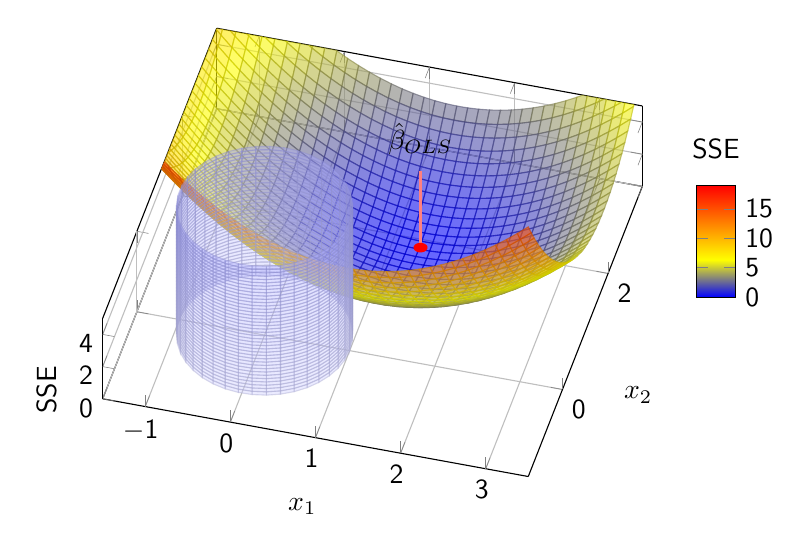
\begin{tikzpicture}
\begin{axis}[
    view={15}{75},
    enlargelimits=false,
    grid=major,
    domain=-1.5:3.5,
    y domain=-1.5:3.5,
    xmin = -1.5,
    ymin = -1.5,
    samples=40,
    zmin=0,
    zmax=5,
    xlabel=$x_1$,
    ylabel=$x_2$,
    zlabel={SSE},
    scaled z ticks=false,
    colorbar,
    colorbar style={
        at={(1.1,0.4)},
        anchor=south west,
        height=0.25*\pgfkeysvalueof{/pgfplots/parent axis height},
        scaled ticks=false,
        title={SSE}
    }
]

\addplot3[surf, opacity=0.6] {(x - 1.35)^2 + (y - 1.8)^2};  % Paraboloid representing the error surface

% \addplot3 [fill=gray!20, opacity=0.7, draw=none, domain=-1:1, samples=40] (x, y, {(x+y)/2 + 2.5}); % L1 constraint (diamond shape)
% L2 constraint - Cylinder for Ridge Regression
\addplot3[surf, domain=0:2*pi, y domain=0:8, colormap={grays}{color(0cm)=(blue!20); color(1cm)=(blue!50)}, opacity = .4, samples=40, z buffer=sort]
  ({cos(deg(x))},{sin(deg(x))},y);

\draw [red!50, thick] (axis cs:1.35,1.8,0) -- (axis cs:1.35,1.8,5); % Line pointing to the minima
\fill[red] (axis cs:1.35,1.8,.25) circle (0.08); % Optimal point on the surface
\node at (axis cs: 1.35, 1.8, 7) {$\hat \beta_{OLS}$};

\end{axis}
\end{tikzpicture}

\end{document}
